\section{光谱表示}\label{sec:光谱表示}

真实世界物体的SPD可能极其复杂;
\reffig{5.1}展示了荧光灯发光的频谱分布和柠檬皮反射率的频谱分布图。
用SPD做计算的渲染器需要紧实、高效且准确的方式表示像这样的函数。
实践中,可能需要在这些特性间作取舍。
\begin{figure}[htbp]
    \centering
    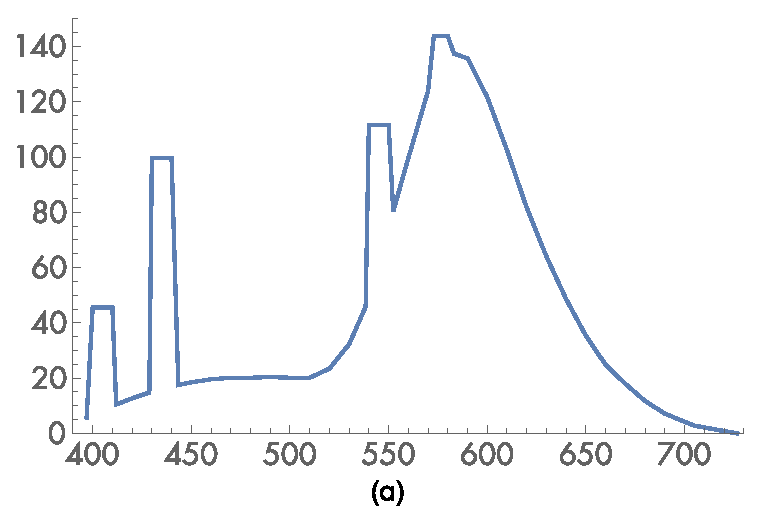
\includegraphics[width=0.45\linewidth]{chap05/fluorescent-spd.eps}\,\nolinebreak
    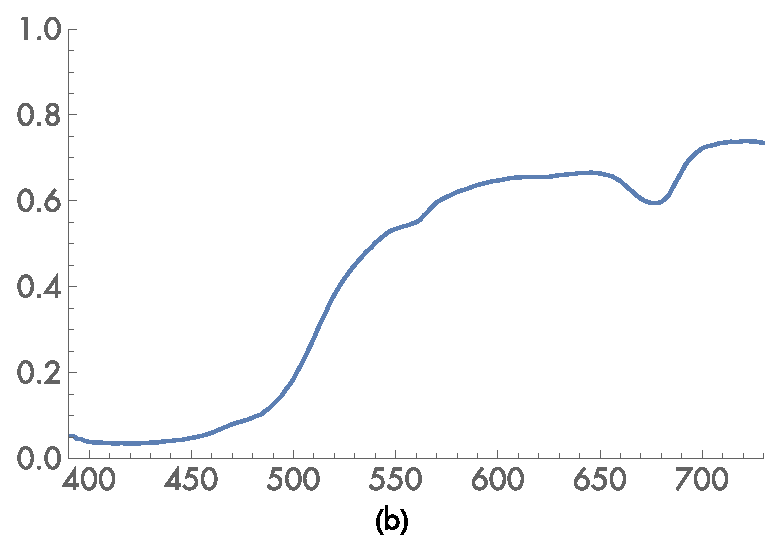
\includegraphics[width=0.45\linewidth]{chap05/lemonskin-spd.eps}
    \caption{(a)荧光灯的频谱分布和(b)柠檬皮的反射率。
        波长400nm左右是偏蓝光,而波长中段是绿色和黄色,波长700nm左右是红光。
        荧光灯的SPD甚至比这里展示的更加尖锐,SPD可归入到10nm范围内;
        它实际上是在单个离散频率上发出大量光。}
    \label{fig:5.1}
\end{figure}

研究这些问题的一般框架可以基于寻找
优良\keyindex{基函数}{basis function}{}以表示SPD的问题来开发。
基函数背后的思想是将可能的SPD函数的无限维空间映射到系数$c_i\in\mathbb{R}$的低维空间。
例如,一个平凡的基函数是常函数$B(\lambda)=1$。
任意SPD可以用等于其平均值的单个系数$c$以该基表示,
这样其近似就为$cB(\lambda)=c$。
很明显这是个很差的近似,因为大多数SPD都比这单个基函数所能准确表示的复杂得多。

在计算机图形学中已经为光谱表示研究了许多不同的基函数;
“扩展阅读”一节引用了关于该话题的许多文献和更多资源。
不同基函数集在关键运算上能提供截然不同的取舍,例如
将任意SPD转换为系数集(将其投影到基上)、
为由基表示的两个SPD之积给定的SPD计算系数等。
本章中,我们将介绍pbrt中可用于光谱的两种表示:\refvar{RGBSpectrum}{},
它遵循经典计算机图形学实践中用表示红、绿和蓝色混合的系数来表示SPD的做法,
以及\refvar{SampledSpectrum}{},它将SPD表示为在一个波长范围上采样点集。

\subsection{光谱类型}\label{sub:光谱类型}
整个pbrt中,我们都根据\refvar{Spectrum}{}类型
用一组特定内建运算符(加法、乘法等)仔细实现涉及SPD的全部计算。
\refvar{Spectrum}{}类型隐藏了所用特定光谱表示的细节,
这样改变系统的这些细节只需要改变\refvar{Spectrum}{}的实现;其他代码可保存不变。
\refvar{Spectrum}{}类型的实现在文件\href{https://github.com/mmp/pbrt-v3/blob/master/src/core/spectrum.h}{\ttfamily core/spectrum.h}和
\href{https://github.com/mmp/pbrt-v3/blob/master/src/core/spectrum.cpp}{\ttfamily core/spectrum.cpp}中。

pbrt中为\refvar{Spectrum}{}类型选择使用哪种光谱表示
在文件\href{https://github.com/mmp/pbrt-v3/blob/master/src/core/pbrt.h}{\ttfamily core/pbrt.h}中
由{\ttfamily typedef}完成。
pbrt默认使用更高效但不太精确的RGB表示。
\begin{lstlisting}
`\initcode{Global Forward Declarations}{=}\initnext{GlobalForwardDeclarations}`
typedef `\refvar{RGBSpectrum}{}` `\initvar{Spectrum}{}`;
// typedef \refvar{SampledSpectrum}{} Spectrum;
\end{lstlisting}

我们还没有把系统编写成在运行时解析选用哪个\refvar{Spectrum}{}表示;
为了切换到不同的表示,整个系统必须重新编译。
这一设计的一个优点是许多各种\refvar{Spectrum}{}方法可以实现为
能被编译器内联\sidenote{译者注:原文inlined。}的短函数,而不是弄成
需要通过相对较慢的虚拟方法调用机制唤起的独立运行函数。
内联像这样的常用短函数能给出性能上的巨大提升。
第二个优点是系统中持有\refvar{Spectrum}{}类型实例的结构可以直接保有它们
而不用在运行时基于所选的光谱表示动态地分配它们。

\subsection{系数光谱实现}\label{sub:系数光谱实现}
本章实现的两种表示都基于排序固定数目的SPD样本。
因此,我们从定义模板类\refvar{CoefficientSpectrum}{}开始,
它将光谱表示为作为模板\refvar{nSpectrumSamples}{}
参数给出的特定数量的样本。
\refvar{RGBSpectrum}{}和\refvar{SampledSpectrum}{}的部分实现都继承自\refvar{CoefficientSpectrum}{}。
\begin{lstlisting}
`\initcode{Spectrum Declarations}{=}\initnext{SpectrumDeclarations}`
template <int `\initvar{nSpectrumSamples}{}`> class `\initvar{CoefficientSpectrum}{}` {
public:
    `\refcode{CoefficientSpectrum Public Methods}{}`
    `\refcode{CoefficientSpectrum Public Data}{}`
protected:
    `\refcode{CoefficientSpectrum Protected Data}{}`
};
\end{lstlisting}
提供了一个\refvar{CoefficientSpectrum}{}构造函数;
它将光谱初始化为所有波长上都是常值。
\begin{lstlisting}
`\initcode{CoefficientSpectrum Public Methods}{=}\initnext{CoefficientSpectrumPublicMethods}`
`\refvar{CoefficientSpectrum}{}`(`\refvar{Float}{}` v = 0.f) {
    for (int i = 0; i < `\refvar{nSpectrumSamples}{}`; ++i)
        `\refvar[CoefficientSpectrum::c]{c}{}`[i] = v;
}
\end{lstlisting}
\begin{lstlisting}
`\initcode{CoefficientSpectrum Protected Data}{=}`
`\refvar{Float}{}` `\initvar[CoefficientSpectrum::c]{c}{}`[`\refvar{nSpectrumSamples}{}`];
\end{lstlisting}
需要针对\refvar{Spectrum}{}对象的各种算术运算符;
\refvar{CoefficientSpectrum}{}中的实现都很简单。
首先,我们定义把光谱分布对加起来的运算符。
对于采样的表示,很容易证明两个SPD之和的每个样本值等于相应样本值之和。
\begin{lstlisting}
`\refvar{CoefficientSpectrum Public Methods}{+=}\lastnext{CoefficientSpectrumPublicMethods}`
`\refvar{CoefficientSpectrum}{}` &operator+=(const `\refvar{CoefficientSpectrum}{}` &s2) {
    for (int i = 0; i < `\refvar{nSpectrumSamples}{}`; ++i)
        `\refvar[CoefficientSpectrum::c]{c}{}`[i] += s2.`\refvar[CoefficientSpectrum::c]{c}{}`[i];
    return *this;
}
\end{lstlisting}
\begin{lstlisting}
`\refvar{CoefficientSpectrum Public Methods}{+=}\lastnext{CoefficientSpectrumPublicMethods}`
`\refvar{CoefficientSpectrum}{}` operator+(const `\refvar{CoefficientSpectrum}{}` &s2) const {
    `\refvar{CoefficientSpectrum}{}` ret = *this;
    for (int i = 0; i < `\refvar{nSpectrumSamples}{}`; ++i)
        ret.`\refvar[CoefficientSpectrum::c]{c}{}`[i] += s2.`\refvar[CoefficientSpectrum::c]{c}{}`[i];
    return ret;
}
\end{lstlisting}

类似地,减法、乘法、除法以及一元取负都按分量定义。
这些方法非常类似于已经展示的那些,所以我们这里不再介绍了。
pbrt也提供了相等和不等测试,这里也不介绍了。

知道光谱是否表示的是一个处处取零值的SPD常常很有用。
例如,如果一个曲面有零反射率,则光线传输例程可以避免
投射最终其作用会被乘以零故不用被追踪的反射光线的计算开销。
\begin{lstlisting}
`\refcode{CoefficientSpectrum Public Methods}{+=}\lastnext{CoefficientSpectrumPublicMethods}`
bool `\initvar{IsBlack}{}`() const {
    for (int i = 0; i < `\refvar{nSpectrumSamples}{}`; ++i)
        if (`\refvar[CoefficientSpectrum::c]{c}{}`[i] != 0.) return false;
    return true;
}
\end{lstlisting}

\refvar{Spectrum}{}的实现(进而与\refvar{CoefficientSpectrum}{}的实现)
必须也提供大量稍微深奥的方法,包括取SPD的平方根或让函数按指定的幂乘方。
例如第\refchap{反射模型}中类\refvar{Fresnel}{}执行的一些计算需要它们。
\refvar[CoefficientSpectrum::Sqrt]{Sqrt}{()}的实现取每个分量的平方根来给出SPD的平方根。
\refvar[CoefficientSpectrum::Pow]{Pow}{()}和\refvar[CoefficientSpectrum::Exp]{Exp}{()}类似,这里就不介绍了。
\begin{lstlisting}
`\refcode{CoefficientSpectrum Public Methods}{+=}\lastnext{CoefficientSpectrumPublicMethods}`
friend `\refvar{CoefficientSpectrum}{}` `\initvar[CoefficientSpectrum::Sqrt]{Sqrt}{}`(const `\refvar{CoefficientSpectrum}{}` &s) { 
    `\refvar{CoefficientSpectrum}{}` ret;
    for (int i = 0; i < `\refvar{nSpectrumSamples}{}`; ++i)
        ret.`\refvar[CoefficientSpectrum::c]{c}{}`[i] = std::sqrt(s.`\refvar[CoefficientSpectrum::c]{c}{}`[i]);
    return ret;
}
\end{lstlisting}

能用参数$t$在两个SPD间线性插值也常常很有用。
\begin{lstlisting}
`\initcode{Spectrum Inline Functions}{=}`
inline `\refvar{Spectrum}{}` `\initvar[Spectrum::Lerp]{Lerp}{}`(`\refvar{Float}{}` t, const `\refvar{Spectrum}{}` &s1, const `\refvar{Spectrum}{}` &s2) {
    return (1 - t) * s1 + t * s2;
}
\end{lstlisting}

图像处理管道的一些部分想要钳位光谱以保证它表示的函数在某允许范围内。
\begin{lstlisting}
`\refcode{CoefficientSpectrum Public Methods}{+=}\lastnext{CoefficientSpectrumPublicMethods}`
`\refvar{CoefficientSpectrum}{}` `\initvar[CoefficientSpectrum::Clamp]{Clamp}{}`(`\refvar{Float}{}` low = 0, `\refvar{Float}{}` high = `\refvar{Infinity}{}`) const {
    `\refvar{CoefficientSpectrum}{}` ret;
    for (int i = 0; i < `\refvar{nSpectrumSamples}{}`; ++i)
        ret.`\refvar[CoefficientSpectrum::c]{c}{}`[i] = ::`\refvar{Clamp}{}`(`\refvar[CoefficientSpectrum::c]{c}{}`[i], low, high);
    return ret;
}
\end{lstlisting}

最后,我们提供一个调试例程来检查SPD是否有任何样本值为not-a-number(NaN浮点值)。
该情况可能因为意外除以0而发生;整个系统的\refvar{Assert}{()}
用该方法在其发生处附近捕获该情况。
\begin{lstlisting}
`\refcode{CoefficientSpectrum Public Methods}{+=}\lastnext{CoefficientSpectrumPublicMethods}` 
bool `\initvar[CoefficientSpectrum::HasNaNs]{HasNaNs}{}`() const {
    for (int i = 0; i < `\refvar{nSpectrumSamples}{}`; ++i)
        if (std::isnan(`\refvar[CoefficientSpectrum::c]{c}{}`[i])) return true;
    return false;
}
\end{lstlisting}

pbrt中绝大多数光谱计算都可用目前我们已经定义的基本运算实现。
然而,一些情况需要能在一组表示SPD的光谱样本上迭代——
例如执行光谱基于样本的表查询或逐波长计算分段函数。
pbrt中需要该功能的类包括用于次表面散射的\refvar{TabulatedBSSRDF}{},
以及类\refvar{HomogeneousMedium}{}和\refvar{GridDensityMedium}{}。

针对这些用途,\refvar{CoefficientSpectrum}{}提供了公有常数\refvar[CoefficientSpectrum::nSamples]{nSamples}{},
它给出用于表示SPD的样本数量,以及方法{\ttfamily operator[]}来获取单个样本值。
\begin{lstlisting}
`\initcode{CoefficientSpectrum Public Data}{=}`
static const int `\initvar[CoefficientSpectrum::nSamples]{nSamples}{}` = `\refvar{nSpectrumSamples}{}`;
\end{lstlisting}
\begin{lstlisting}
`\refcode{CoefficientSpectrum Public Methods}{+=}\lastcode{CoefficientSpectrumPublicMethods}`
`\refvar{Float}{}` &operator[](int i) {
    return `\refvar[CoefficientSpectrum::c]{c}{}`[i];
}
\end{lstlisting}

注意该样本获取器的存在利用了隐含假设即
光谱表示是线性缩放一组固定基函数的一组系数。
例如如果一个\refvar{Spectrum}{}实现改为用高斯函数和表示SPD,
其中系数$c_i$交替缩放高斯函数并设置其宽度,
\begin{align*}
    S(\lambda)=\sum\limits_i^N{c_{2i}\mathrm{e}^{-c_{2i+1}}}\, ,
\end{align*}
则当前使用该获取器的代码需要做修改,以替代把SPD转换为一组线性系数的版本。
尽管在\refvar{Spectrum}{}抽象中该尝试并不完美,
但它简化了当前系统的其他部分,且如果添加该假设不成立的光谱表示,清理起来也不会太难。